\documentclass[tikz,border=10pt]{standalone}
\usepackage{amsmath}
\usetikzlibrary{arrows.meta, positioning, calc, decorations.pathreplacing}
\definecolor{c1}{HTML}{000000}
\definecolor{c2}{HTML}{233D4D}
\definecolor{c3}{HTML}{FE7F2D}
\definecolor{c4}{HTML}{EAECF0}
\definecolor{labelcolor}{HTML}{5F6B75}
\begin{document}
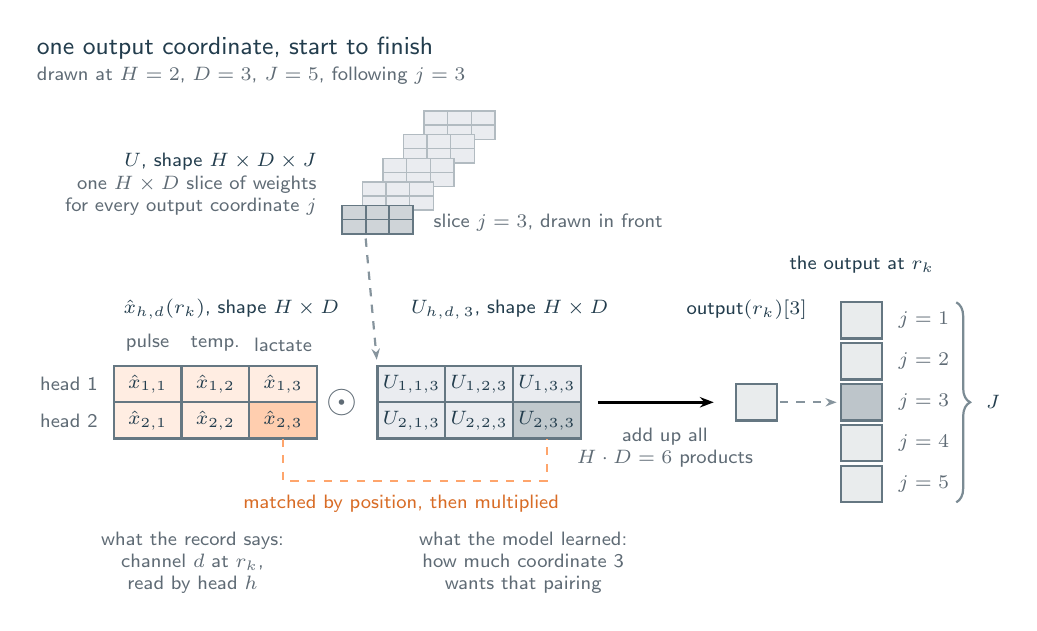
\begin{tikzpicture}[
    every node/.style={font=\sffamily},
    lab/.style={font=\sffamily\scriptsize, text=labelcolor},
    tag/.style={font=\sffamily\scriptsize, text=c2},
    hot/.style={font=\sffamily\scriptsize, text=c3!85!black},
    xc/.style={rectangle, draw=c2!70, fill=c3!14, line width=0.8pt,
               minimum width=0.86cm, minimum height=0.46cm,
               font=\sffamily\scriptsize, text=c2, inner sep=1pt},
    xh/.style={xc, fill=c3!38},
    uc/.style={rectangle, draw=c2!70, fill=c4, line width=0.8pt,
               minimum width=0.86cm, minimum height=0.46cm,
               font=\sffamily\scriptsize, text=c2, inner sep=1pt},
    uh/.style={uc, fill=c2!28},
    ocell/.style={rectangle, draw=c2!70, fill=c2!10, line width=0.8pt,
                  minimum width=0.52cm, minimum height=0.46cm},
    oh/.style={ocell, fill=c2!30},
    arr/.style={-{Stealth[length=5pt]}, line width=1.0pt, color=c1},
    gd/.style={-{Stealth[length=4pt]}, line width=0.8pt, color=c2!55, dashed},
]

\node[tag, anchor=west, font=\sffamily\small] at (0.30, 7.60)
     {one output coordinate, start to finish};
\node[lab, anchor=west] at (0.30, 7.25)
     {drawn at $H = 2$, $D = 3$, $J = 5$, following $j = 3$};

% ================================================== the tensor U, as a stack
\foreach \s in {4,3,2,1}{
  \foreach \r in {0,1}{ \foreach \c in {0,1,2}{
    \draw[draw=c2!35, fill=c4, line width=0.5pt]
      ({4.30+\s*0.26+\c*0.30}, {5.60+\s*0.30-\r*0.18-0.18})
      rectangle ({4.30+\s*0.26+\c*0.30+0.30}, {5.60+\s*0.30-\r*0.18});}}}
\foreach \r in {0,1}{ \foreach \c in {0,1,2}{
  \draw[draw=c2!70, fill=c2!22, line width=0.6pt]
    ({4.30+\c*0.30}, {5.60-\r*0.18-0.18})
    rectangle ({4.30+\c*0.30+0.30}, {5.60-\r*0.18});}}

\node[tag, anchor=east] at (4.10, 6.15) {$U$, shape $H \times D \times J$};
\node[lab, anchor=east, align=right] at (4.10, 5.72)
     {one $H \times D$ slice of weights\\ for every output coordinate $j$};
\node[lab, anchor=west] at (5.34, 5.38) {slice $j = 3$, drawn in front};

\draw[gd] (4.60, 5.18) -- (4.74, 3.64);

% ============================================ block 1: the interpolations
\node[tag, anchor=west] at (1.40, 4.28) {$\hat{x}_{h,d}(r_k)$, shape $H \times D$};
\foreach \d/\x/\name in {1/1.83/{pulse}, 2/2.69/{temp.}, 3/3.55/{lactate}}{
  \node[lab, anchor=south] at (\x, 3.62) {\name};}
\foreach \h/\y in {1/3.33, 2/2.87}{
  \node[lab, anchor=east] at (1.32, \y) {head \h};}
\node[xc] at (1.83, 3.33) {$\hat{x}_{1,1}$};
\node[xc] at (2.69, 3.33) {$\hat{x}_{1,2}$};
\node[xc] at (3.55, 3.33) {$\hat{x}_{1,3}$};
\node[xc] at (1.83, 2.87) {$\hat{x}_{2,1}$};
\node[xc] at (2.69, 2.87) {$\hat{x}_{2,2}$};
\node[xh] at (3.55, 2.87) {$\hat{x}_{2,3}$};

\node[font=\sffamily\Large, text=labelcolor] at (4.30, 3.10) {$\odot$};

% ============================================ block 2: the slice of U
\node[tag, anchor=west] at (5.05, 4.28) {$U_{h,d,\,3}$, shape $H \times D$};
\node[uc] at (5.18, 3.33) {$U_{1,1,3}$};
\node[uc] at (6.04, 3.33) {$U_{1,2,3}$};
\node[uc] at (6.90, 3.33) {$U_{1,3,3}$};
\node[uc] at (5.18, 2.87) {$U_{2,1,3}$};
\node[uc] at (6.04, 2.87) {$U_{2,2,3}$};
\node[uh] at (6.90, 2.87) {$U_{2,3,3}$};

% the elementwise pairing, shown once
\draw[c3!70, line width=0.9pt, dashed]
     (3.55, 2.64) -- (3.55, 2.10) -- (6.90, 2.10) -- (6.90, 2.64);
\node[hot, anchor=north] at (5.05, 2.04)
     {matched by position, then multiplied};

% ============================================ block 3: the sum
\draw[arr] (7.55, 3.10) -- (9.02, 3.10);
\node[lab, anchor=north, align=center] at (8.40, 2.90)
     {add up all\\ $H \cdot D = 6$ products};
\node[tag, anchor=west] at (8.55, 4.28) {$\text{output}(r_k)[3]$};
\node[ocell] at (9.56, 3.10) {};

\draw[gd] (9.86, 3.10) -- (10.58, 3.10);

% ============================================ the output vector
\node[tag, anchor=south] at (10.90, 4.62) {the output at $r_k$};
\foreach \j in {1,...,5}{
  \pgfmathsetmacro\yy{4.14 - (\j-1)*0.52}
  \ifnum\j=3
    \node[oh] at (10.90, \yy) {};
  \else
    \node[ocell] at (10.90, \yy) {};
  \fi
  \node[lab, anchor=west] at (11.24, \yy) {$j = \j$};}
\draw[decorate, decoration={brace, amplitude=5pt}, c2!60, line width=0.8pt]
     (12.10, 4.37) -- (12.10, 1.83)
     node[midway, right=7pt, font=\sffamily\scriptsize, text=c2] {$J$};

% ============================================ what the two grids hold
\node[lab, anchor=north, align=center] at (2.40, 1.58)
     {what the record says:\\ channel $d$ at $r_k$,\\ read by head $h$};
\node[lab, anchor=north, align=center] at (6.60, 1.58)
     {what the model learned:\\ how much coordinate 3\\ wants that pairing};

\end{tikzpicture}
\end{document}
